\documentclass[12pt, a4paper]{article}
\usepackage[british]{babel}
\usepackage[latin1]{inputenc}
\usepackage{amsmath}
\usepackage{amssymb}
\usepackage{booktabs}
\usepackage{pgfplots}
\pgfplotsset{/pgf/number format/use comma,compat=newest}

\title{\textbf{Convergence tests}}
\author{Andrea Vescovini}
\date{\today}

\begin{document}
	\maketitle
\section{Short introduction}

I solved with SIP-DGFEM the Poisson problem with Dirichlet boundary conditions in a cubic domain $\Omega = [0,1]^{3} \subset \mathbb{R}^{3} $ partitioned in $M$ disjoint polyhedral elements $\Omega_{m}$ such that. $\bigcup\limits_{m=1}^{M} \Omega_{m} $.\\
I chose the basis as in \cite{hpmet}. Firstly for every element $\Omega_m$ I constructed a Cartesian bounding box $B_m = I^1_m \times I^2_m \times I^3_m $ such that $\overline{\Omega_m} \subseteq \overline{B_m}$, then for every $B_m$ I defined a standard polynomial space $\mathbf{P}_r(B_m)$, spanned by Legendre tensor-product basis functions $ \{ \phi_{m,i} \}_{i=1}^{dim(\mathbf{P}_r(B_m))} $:
\begin{equation*}
\phi_{m,i}(x,y,z) = L_{r_1}^{[1]}(x)L_{r_2}^{[2]}(y)L_{r_3}^{[3]}(z) \; \; \; \;
r_1+r_2+r_3 \leq r, \; r_k \geq 0, \; k = 1,2,3.
\end{equation*}
where $L_{r_k}^{[d]} $ is the scaled Legendre polynomial over the interval $ I^d $ of degree $ r_k $.\\
I chose the penalization parameter $\sigma $ as in \cite{multigrid}:
\begin{equation}
\sigma ( \mathbf{x} ) = 
\begin{cases}
C_\sigma \max\limits_{\Omega_m \in \{ \Omega_m^{+}, \Omega_m^{-} \} }, &\text{ if $ x \in F, \; F \subset \partial \Omega_m^{+} \cap \partial \Omega_m^{-} $ }\\
C_\sigma \frac{r^2}{h_m}, &\text{ if $ x \in F, \; F \subset \partial \Omega_m \cap \partial \Omega$}
\end{cases}
\end{equation}
where $h_m$ is the diameter of the element $\Omega_m$, $F$ is a face shared bt $\Omega_m^{+}$ and $\Omega_m^{-}$, $C_{\sigma}$ is a constant that has been taken equal to 10.\\


\newpage
\section{Numerical Experiments}
\subsection{Hexahedral meshes}

I solved the problem over three hexahedral meshes of 8, 64 and 512 elements, with $r = 1,2,3$, choosing the source term $f$ and the Dirichlet data $g_D$ such that the excact solution is $u(x,y,z)= e^{xyz}$. I computed the $L^{2}$-norm and $H^{1}$-seminorm of the approximation error $e_{h} = u - u_{h}$.

\begin{table}[h]
	\centering
\[
\begin{array}{cccccc}
	\toprule
	r & Error & 8 elem & 64 elem & 512 elem & \text{Rate} \\ 
	\midrule
	1 & ||e_{h}||_{L^2} & 2.7755 \times 10^{-2} & 7.3256 \times 10^{-3} & 1.8931 \times 10^{-3} & 1.952172\\
	  & |e_{h}|_{H^1}   & 3.1840 \times 10^{-1} & 1.6678 \times 10^{-1} & 8.4123 \times 10^{-2} & 0.987356\\
	\midrule
	2 & ||e_{h}||_{L^2} & 4.9882 \times 10^{-3} & 6.5314 \times 10^{-4} & 7.9122 \times 10^{-5} & 3.045243\\
	  & |e_{h}|_{H^1}   & 6.9691 \times 10^{-2} & 1.8519 \times 10^{-2} & 4.6362 \times 10^{-3} & 1.997973\\
	\midrule
	3 & ||e_{h}||_{L^2} & 1.0479 \times 10^{-3} & 6.6445 \times 10^{-5} & 3.6604 \times 10^{-6} & 4.182076\\
   	  & |e_{h}|_{H^1}   & 1.6100 \times 10^{-2} & 2.1286 \times 10^{-3} & 2.5782 \times 10^{-4} & 3.045478\\
	\bottomrule
\end{array}
\]
\caption{Errors with respect to $h$-refinement.}
\end{table}

\begin{figure}[h!]
\centering
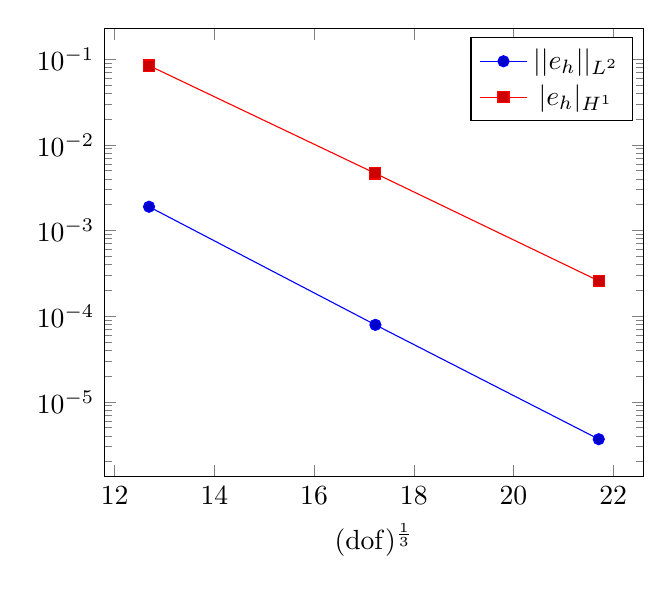
\begin{tikzpicture}
\begin{semilogyaxis}[xlabel={(dof)$^\frac{1}{3}$}]
\addplot coordinates
{(12.69, 1.8931e-3) (17.23, 7.9122e-5) (21.71,3.6604e-6)};
\addplot coordinates
{(12.69, 8.4123e-2) (17.23, 4.6362e-3) (21.71,2.5782e-4)};
\legend{$||e_{h}||_{L^2}$, $|e_{h}|_{H^1}$}
\end{semilogyaxis}
\end{tikzpicture}
\caption{Errors with respect to $p$-refinement computed over the 512 elements mesh.}
\end{figure}

\subsection{Hexahedral-tetrahedral meshes}
Then I solved the same problem over three structured mixed meshes of hexahedra and tetrahedra.

\begin{table}[h]
	\centering
	\[
	\begin{array}{cccccc}
	\toprule
	r & Error & 28 elem & 224 elem & 1792 elem & \text{Rate} \\ 
	\midrule
	1 & ||e_{h}||_{L^2} & 2.5401 \times 10^{-2} & 6.1132 \times 10^{-3} & 1.4851 \times 10^{-3} & 2.041364\\
	  & |e_{h}|_{H^1}   & 3.3681 \times 10^{-1} & 1.8227 \times 10^{-1} & 9.4090 \times 10^{-2} & 0.953993\\
	\midrule
	2 & ||e_{h}||_{L^2} & 4.1276 \times 10^{-3} & 7.0478 \times 10^{-4} & 8.9470 \times 10^{-5} & 2.977697\\
	  & |e_{h}|_{H^1}   & 7.4183 \times 10^{-2} & 1.9944 \times 10^{-2} & 5.0984 \times 10^{-3} & 1.967808\\
	\midrule
	3 & ||e_{h}||_{L^2} & 1.1527 \times 10^{-3} & 7.1514 \times 10^{-5} & 3.9958 \times 10^{-6} & 4.161651\\
	  & |e_{h}|_{H^1}   & 1.8013 \times 10^{-2} & 2.3198 \times 10^{-3} & 2.7689 \times 10^{-4} & 3.066645\\
	\bottomrule
	\end{array}
	\]
	\caption{Errors with respect to $h$-refinement.}
\end{table}

\begin{figure}[h!]
	\centering
	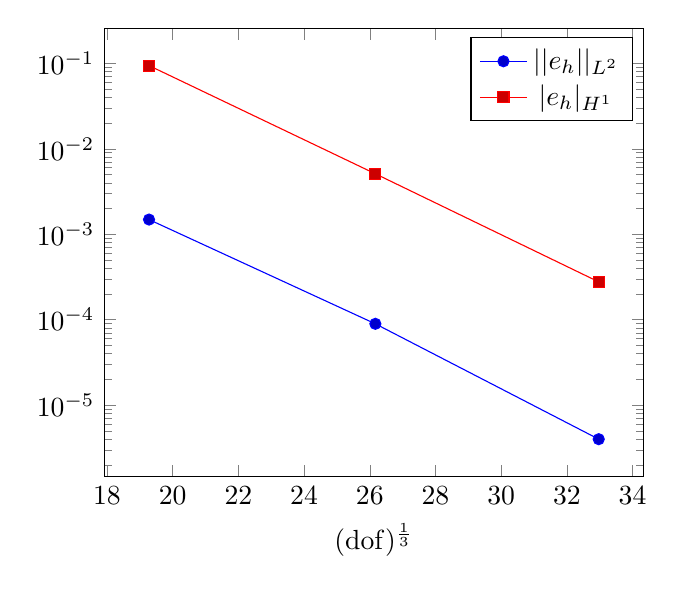
\begin{tikzpicture}
	\begin{semilogyaxis}[xlabel={(dof)$^\frac{1}{3}$}]
	\addplot coordinates
	{(19.28, 1.4851e-3) (26.17, 8.9470e-5) (32.97, 3.9958e-6)};
	\addplot coordinates
	{(19.28, 9.4090e-2) (26.17, 5.0984e-3) (32.97, 2.7689e-4)};
	\legend{$||e_{h}||_{L^2}$, $|e_{h}|_{H^1}$}
	\end{semilogyaxis}
	\end{tikzpicture}
	\caption{Errors with respect to $p$-refinement computed over the 1792 elements mesh.}
\end{figure}

\subsection{General meshes}
Finally I solved the problem over three meshes of arbitrary polyhedra.

\begin{table}[h]
	\centering
	\[
	\begin{array}{cccccc}
	\toprule
	r & Error & 15 elem & 120 elem & 965 elem & \text{Rate} \\ 
	\midrule
	1 & ||e_{h}||_{L^2} & 3.1209 \times 10^{-2} & 1.7716 \times 10^{-2} & 5.9973 \times 10^{-3} & 1.971817\\
	  & |e_{h}|_{H^1}   & 3.5875 \times 10^{-1} & 2.5131 \times 10^{-1} & 1.4168 \times 10^{-1} & 1.043318\\
	\midrule
	2 & ||e_{h}||_{L^2} & 5.3520 \times 10^{-3} & 1.8324 \times 10^{-3} & 2.8963 \times 10^{-4} & 3.358372\\
	  & |e_{h}|_{H^1}   & 8.7963 \times 10^{-2} & 4.2298 \times 10^{-2} & 1.3036 \times 10^{-2} & 2.142675\\
	\midrule
	3 & ||e_{h}||_{L^2} & 1.4164 \times 10^{-3} & 2.2474 \times 10^{-4} & 2.0407 \times 10^{-5} & 4.367402\\
	  & |e_{h}|_{H^1}   & 1.9945 \times 10^{-2} & 6.1835 \times 10^{-3} & 1.1137 \times 10^{-3} & 3.120701\\
	\bottomrule
	\end{array}
	\]
	\caption{Errors with respect to $h$-refinement.}
\end{table}

\begin{figure}[h!]
	\centering
	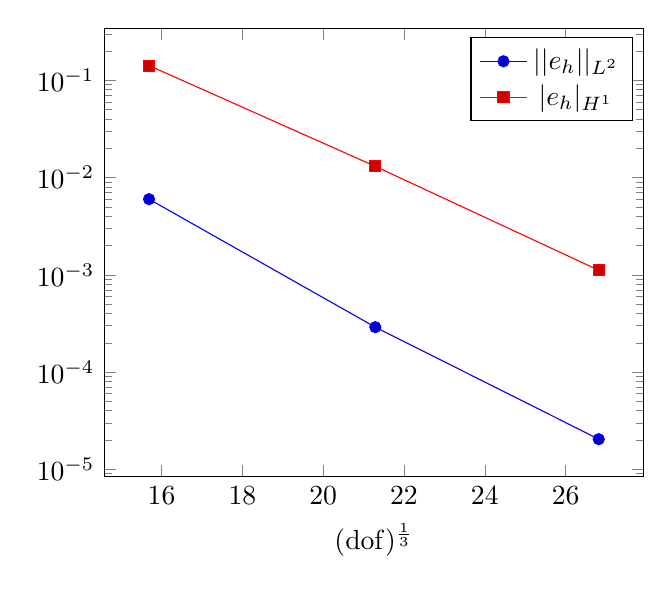
\begin{tikzpicture}
	\begin{semilogyaxis}[xlabel={(dof)$^\frac{1}{3}$}]
	\addplot coordinates
	{(15.69, 5.9973e-3) (21.29, 2.8963e-4) (26.82, 2.0407e-5)};
	\addplot coordinates
	{(15.69, 1.4168e-1) (21.29, 1.3036e-2) (26.82, 1.1137e-3)};
	\legend{$||e_{h}||_{L^2}$, $|e_{h}|_{H^1}$}
	\end{semilogyaxis}
	\end{tikzpicture}
	\caption{Errors with respect to $p$-refinement computed over the 965 elements mesh.}
\end{figure}


\begin{thebibliography}{9}
	\bibitem{hpmet}
	A. Cangiani, E. H. Georgoulis, P. Houston. Hp-Version
	discontinuous Galerkin methods on polygonal and polyhedral meshes. \textit{Mathematical Models and Methods in Applied Sciences}, 2014.
	
	\bibitem{multigrid}
	P. F. Antonietti, P. Houston, X. Hu, M. Sarti, M. Verani. Multigrid algorithms for hp-version interior penalty
	discontinuous Galerkin methods on polygonal and
	polyhedral meshes. \textit{Calcolo}, 2017.
\end{thebibliography}

\end{document}